
\section{Evidencia empírica}
En el artículo original publicado por Boyer y Moore (ver \cite{articulo1}) 
se presentaban los resultados de un test de eficiencia del algoritmo. Se ha considerado pertinente mostrar esos resultados aquí para comprobar de forma empírica la eficiencia del algoritmo.\\

El test selecciona aleatoriamente subpatrones de una secuencia base de caracteres. Se seleccionaron 300 subpatrones para cada longitud de subpatrón entre 1 y 14. Después se utilizaba el algoritmo de Boyer-Moore para buscar coincidencias, empezando desde una posición aleatoria de la primera mitad de la secuencia base. Se midió la eficiencia dividiendo el número de referencias a $y$ entre el número de caracteres de $y$ pasados durante el tiempo de ejecución del algoritmo. Esta medida es independiente de la implementación del algoritmo. Después se realizaría una media aritmética entre las 300 muestras de cada patrón.\\

Como la eficacia del algoritmo dependía de las propiedades estadísticas de $x$ e $y$, se realizó el test para tres textos distintos de 10000 caracteres cada uno. Uno era una secuencia aleatoria de 0's y 1's, otro era un texto en inglés obtenido de un manual online y el tercero era una secuencia aleatoria de caracteres de un diccionario de 100 caracteres. \\

\begin{figure}[H]
  \centering
    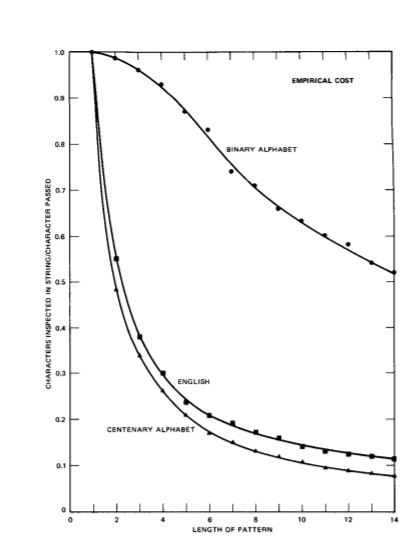
\includegraphics[width=0.45\textwidth]{performance}
	\label{performance}
\end{figure}

Los resultados del test muestran que la eficacia del algoritmo incrementa, para los tres textos, conforme aumenta la longitud del patrón buscado. Vemos que, a partir de los seis caracteres de longitud en los textos no binarios, el algoritmo solo referencia de media uno de cada cinco caracteres de $y$. Además, el ratio caracteres inspeccionados/caracteres pasados siempre es menor a uno (si $x$ consta de más de un carácter), es decir, el algoritmo mejora el coste lineal en estos casos.
